\subsection{Toy example - Synthetic Dataset}
First experiments were run on synthetic data to test its reliability. The workflow allows to build a dataset with custom number of informative features (F), redundant features (R), copies (C) and noise (N). Redundant features are our main aim, and they depend on F features, usually their squared version. The generated values are random and the target is build using only items $\in$ F.
% cuantas muestras? y variables

After swapping, the results (Figure \ref{fig:triade}) show:

\begin{itemize}
    \item Features $\in$ F are not related to each other in the diagram, therefore discriminations performs well.
    \item Copied features behave as expected, since they hold a strong (mutual) relation to their informative features. Again, copies are not related among them.
    \item Redundant features consistent in terms of relation, i.e. they are related to their Original feature’ copies, and other redundant. E.g. R02 to F02, C02 and Cos02.
\end{itemize}

\begin{figure}[!hb]
	\centering
	\begin{subfigure}[b]{0.3\linewidth}
		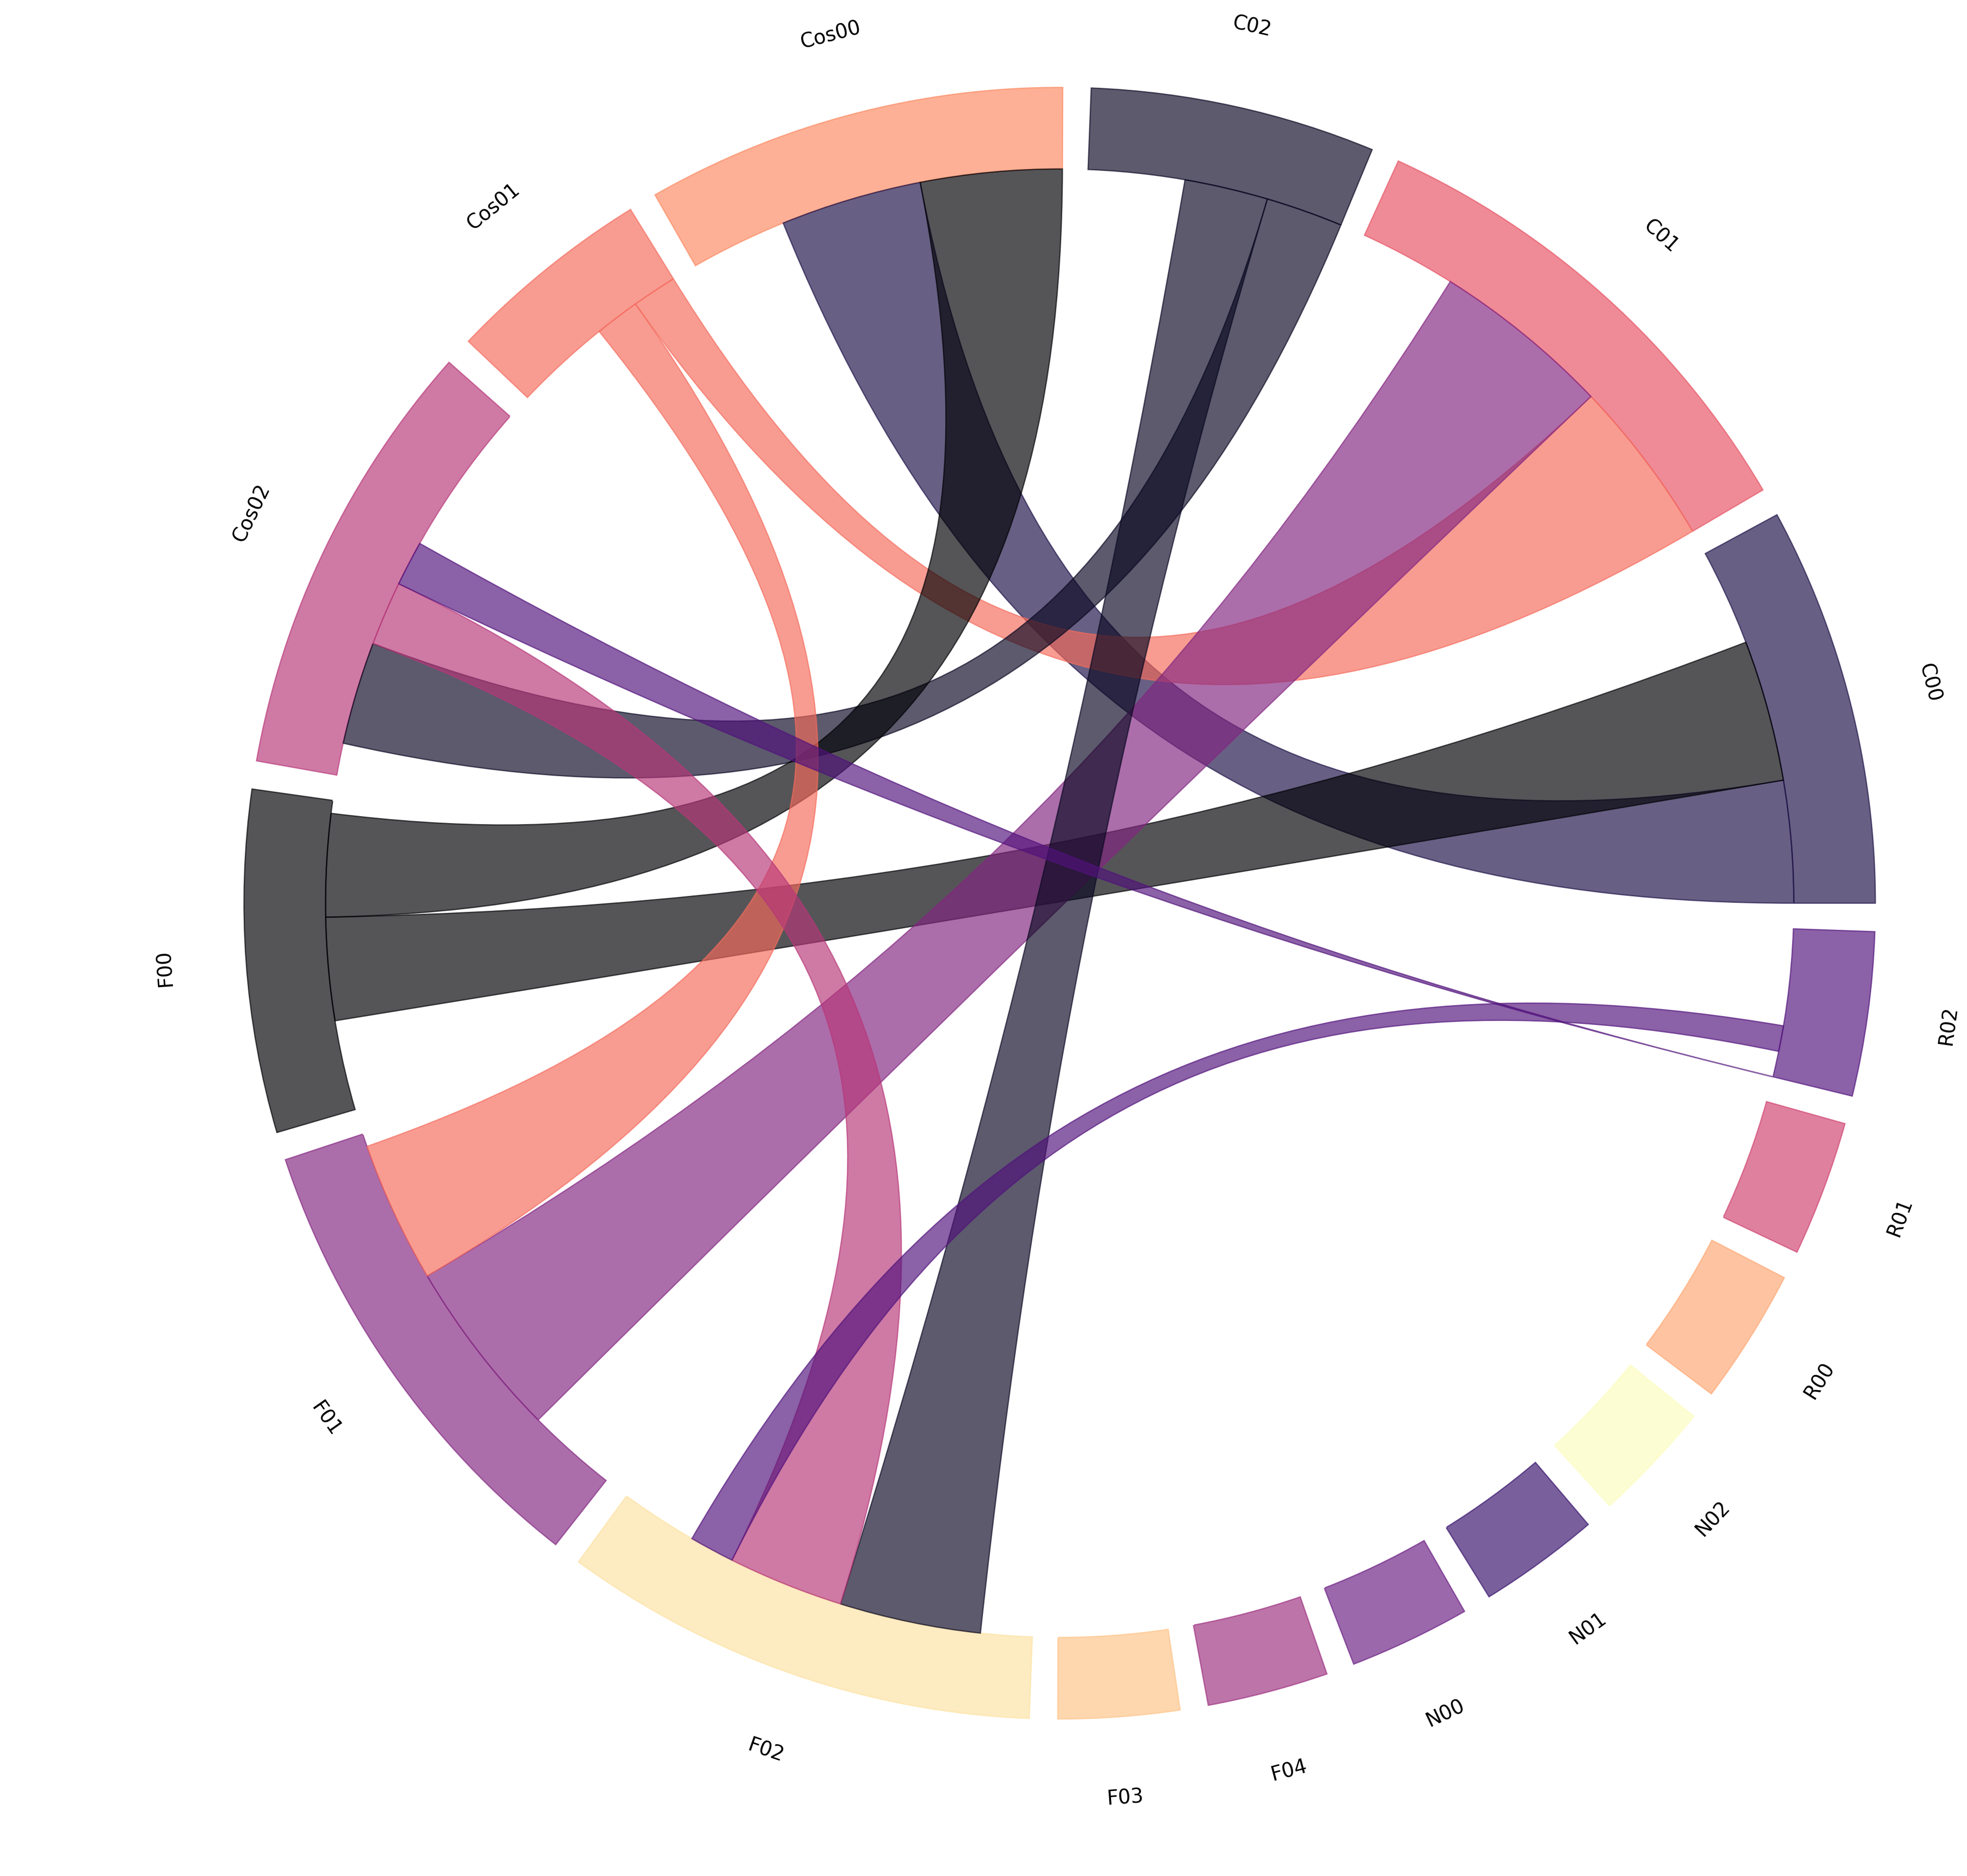
\includegraphics[width=\linewidth]{figures/chords/chord_swap_ensemble1000_RCN5333300_097.png}
		\caption{Chord diagram representation at \emph{t} = 0.98}
	\end{subfigure}
	\hfill
	\begin{subfigure}[b]{0.3\linewidth}
		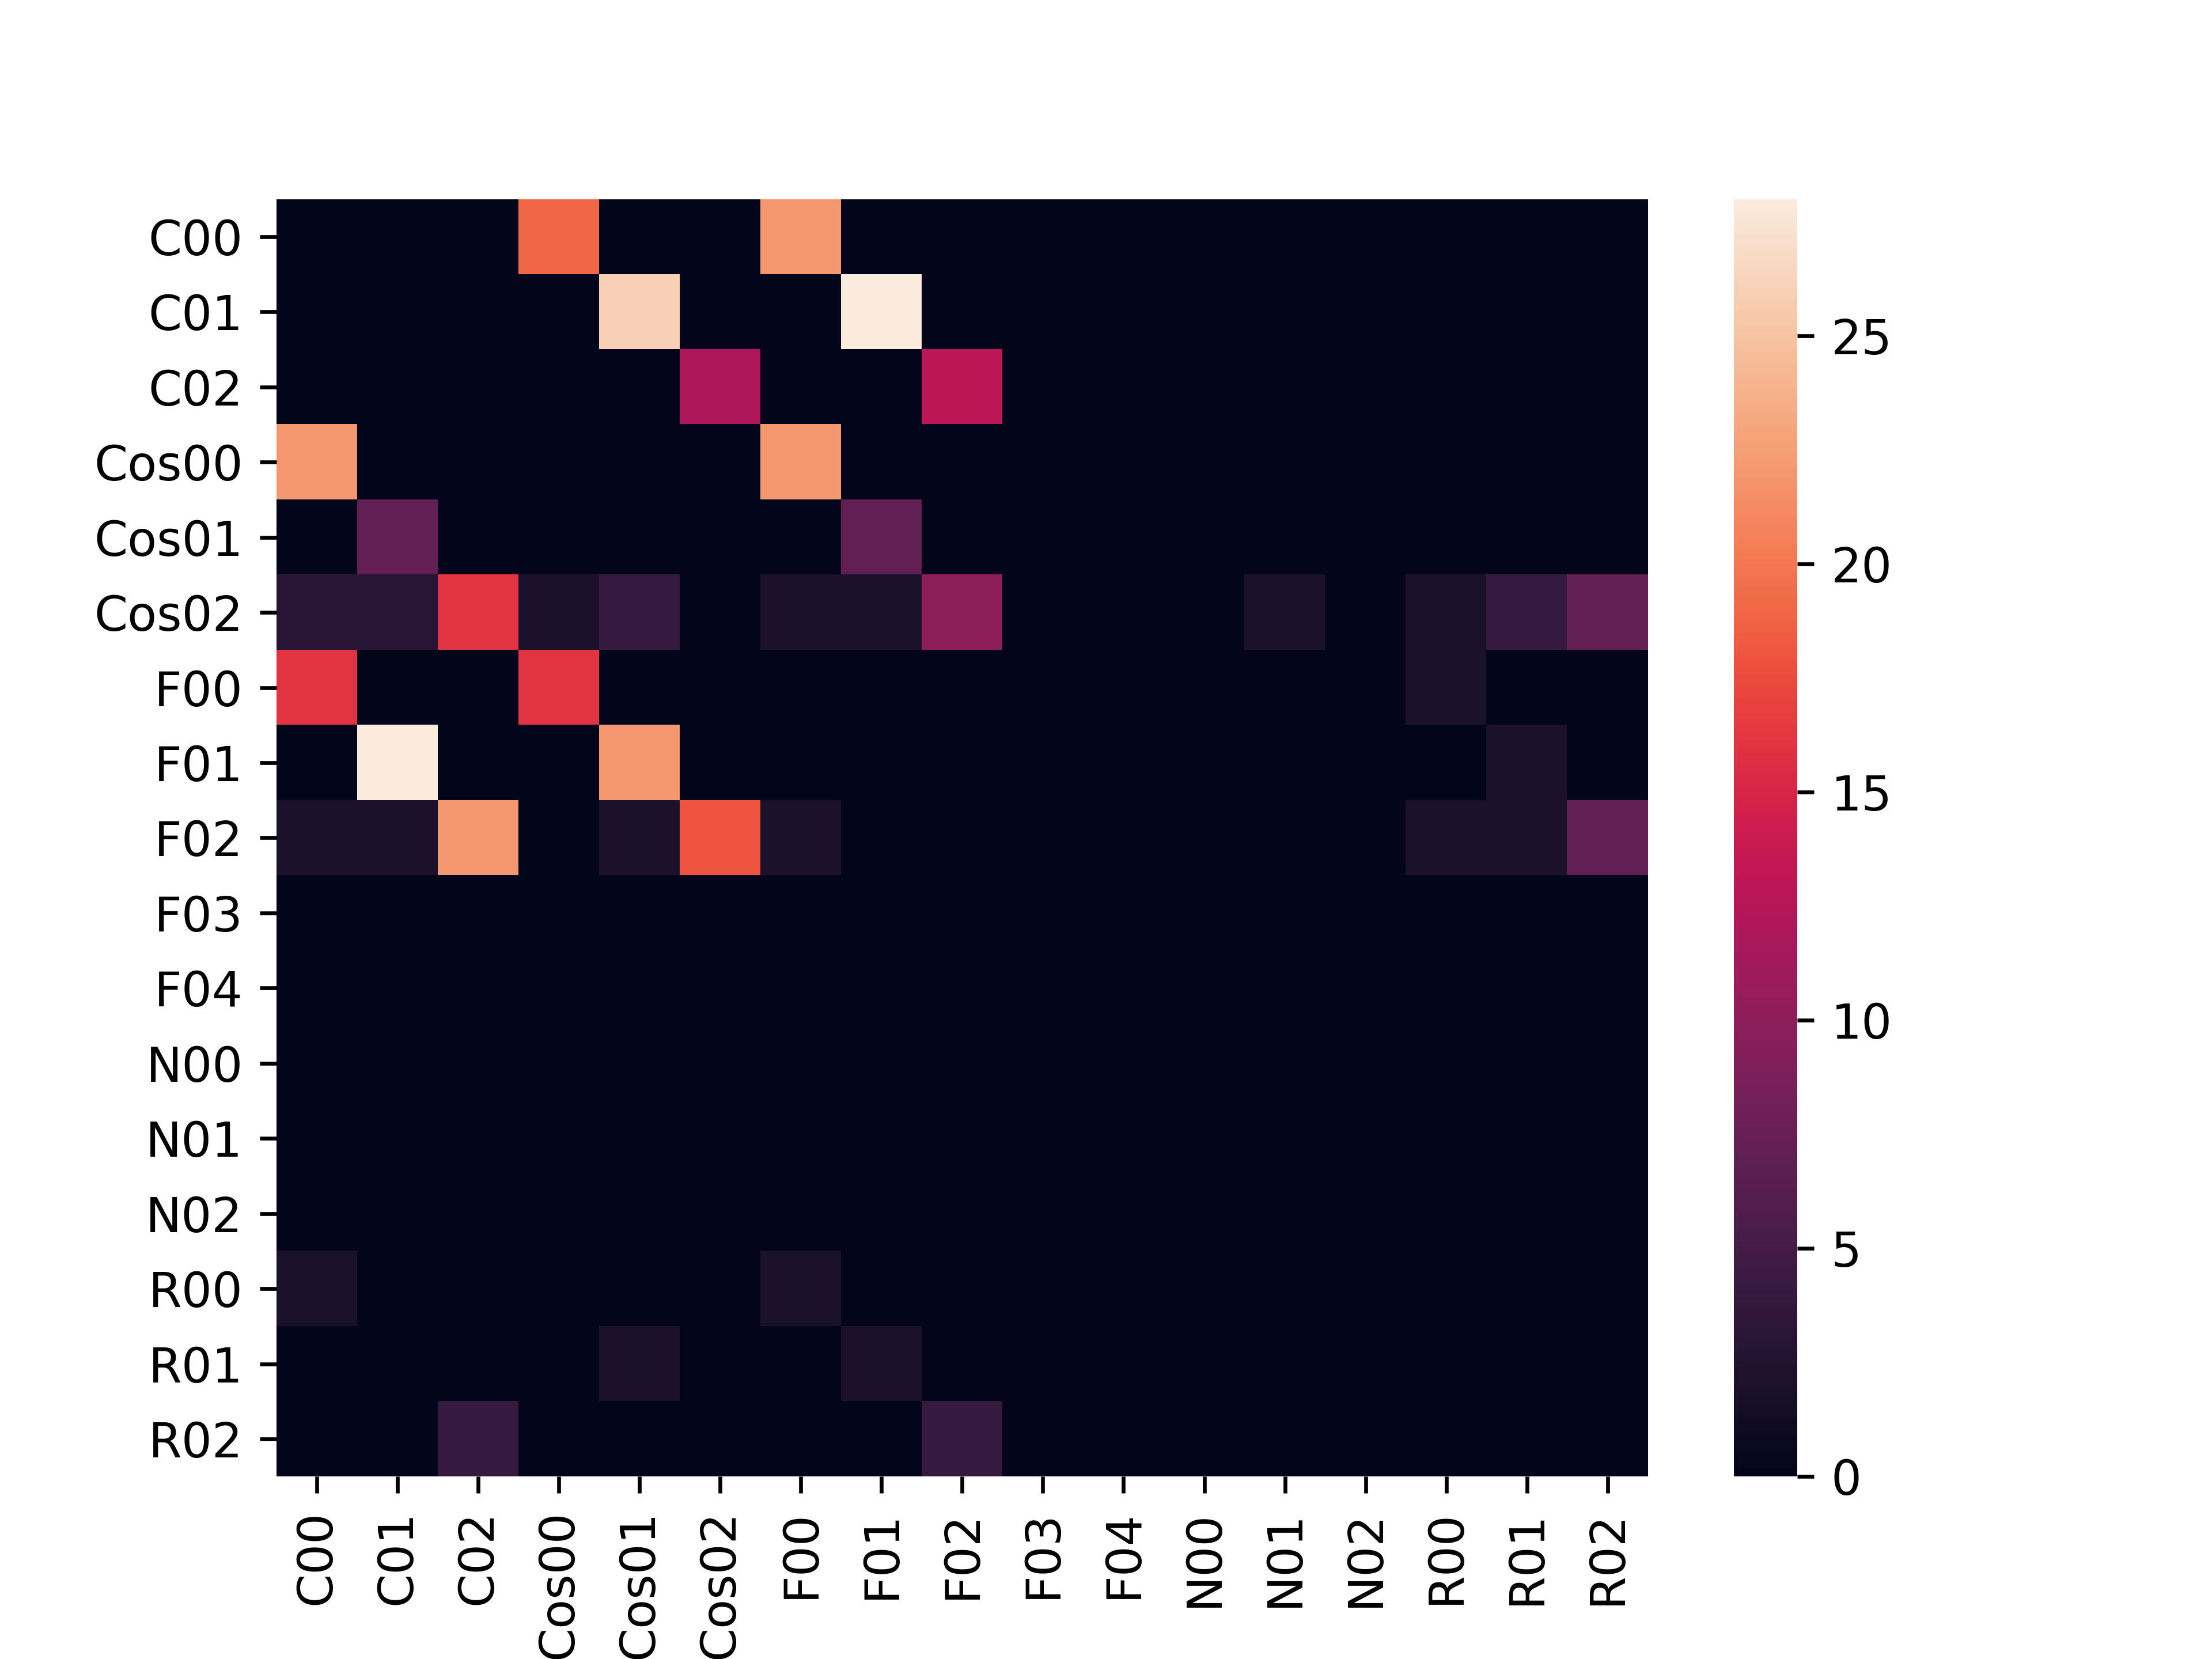
\includegraphics[width=\linewidth]{figures/heatmaps/heatmap_swap_ensemble1000_RCN5333300_097.png}
		\caption{Heatmap from matrix at \emph{t} = 0.98. Edge thickness indicates relation strength.}
	\end{subfigure}
	\hfill
	\begin{subfigure}[b]{0.3\linewidth}
		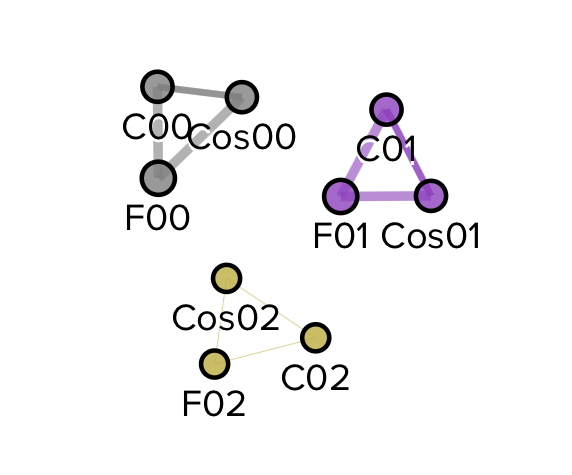
\includegraphics[width=\linewidth]{Minor Thesis/figures/graphs/graph-toy.png}
		\caption{Graph clustering at \emph{t} = 0.98}
	\end{subfigure}
	\caption{Clustering process. (a) Shows relation in Chord diagram to ease visualisation. (b) Gives the matrix which we post-process to keep only relevant links. (c) Final relation graph. Each connected component is a final group whose representative is the most connected node. Community detection algorithms colour each group.}
	\label{fig:triade}
\end{figure}

On the other hand, we also found a drawback: Some redundant features relate to other than theirs. E.g R00 relates to F01, F02. However, the relation is stronger to R00, which can only by filtered by a threshold modification, allowing only relations above 0.97 get past it. Evolution of the relations using a moving threshold can be found in Suppl. Material \ref{suppl:relations}

% mensaje de conclusion: utilizando un dataset perfectamente controlado, hemos podido validar el buen comportamiento del algoritmo. A continuacion se presenta un analisis realizado con datos reales.


\subsection{Type 2 Diabetes - Real Dataset}
Scripts applied to the Type 2 Diabetes (T2D) deliver results which can be interpretable using biological background. At a more in depth level, and taking into account the capabilities of the system, we pay attention not only to the results, but to the kind of data.
\\

A regular swapping run on an ensemble containing T2D data takes 984$\times$3$\times$8$\times$298 = 7,037,568 swap attempts (Eq. in \ref{section:methods:complex}), being 984 the number of sequentials, 3 splits of data each, 8 original variables and 289 top variables to swap.
On completion, we extract the results.
\\

Normalised scores show the following pattern: When plotting the graph step by step -- filtering edge weight from the highest to the lowest-- , the variables added tend to have a $\approx$ 0.98 Spearman Correlation similarity in the original data. Besides, for each addition, we add a node to the connected component and do not form new ones. If any CC is created, it is soon linked. See Suppl. Material \ref{fig:graph-evo-sa} for graph evolution.
\\

Not-normalised scores show the same pattern, except the node additions is more exponential, i.e. it does not add one node at the time, but several.
Testing the similarity score among features by randomly picking them shows a bimodal distribution: either the results are close to 0.9 or to 0.1, which might be causing the bias in the swapper. See Suppl. Material \ref{fig:graph-evo-nn} for graph evolution.
\\

Finally, on normalised scores corrected for quasi-constancy, a majority of CC containing 2 and 3 nodes is found (Figure \ref{fig:main-graphs}). 
\\
\begin{figure}[!ht]
    \centering
% 	\captionsetup{justification=centering}
	\begin{subfigure}[b]{0.30\linewidth}
		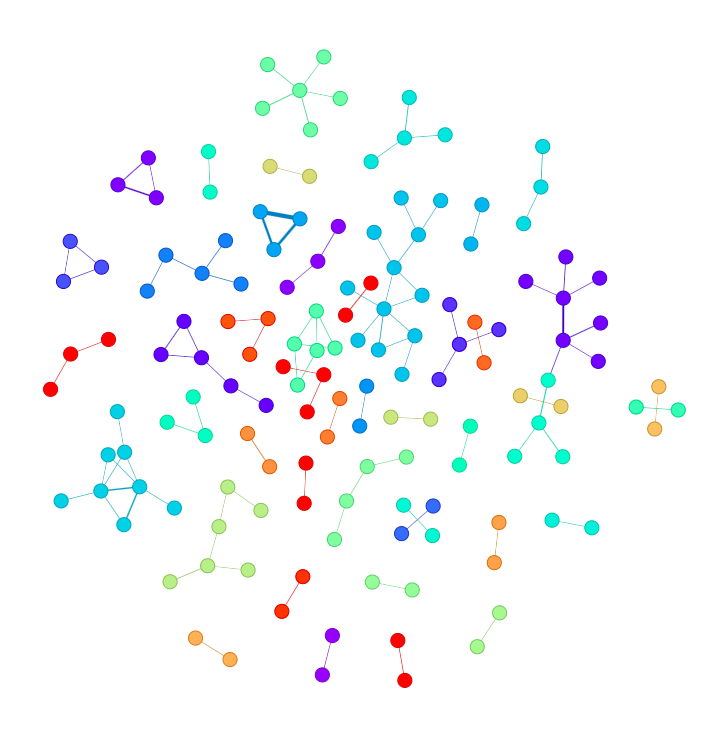
\includegraphics[width=\linewidth]{Minor Thesis/figures/graphs/main/g95102028.png}
		\caption{10\% cases min.}
	\end{subfigure}
	\hfill
	\begin{subfigure}[b]{0.30\linewidth}
		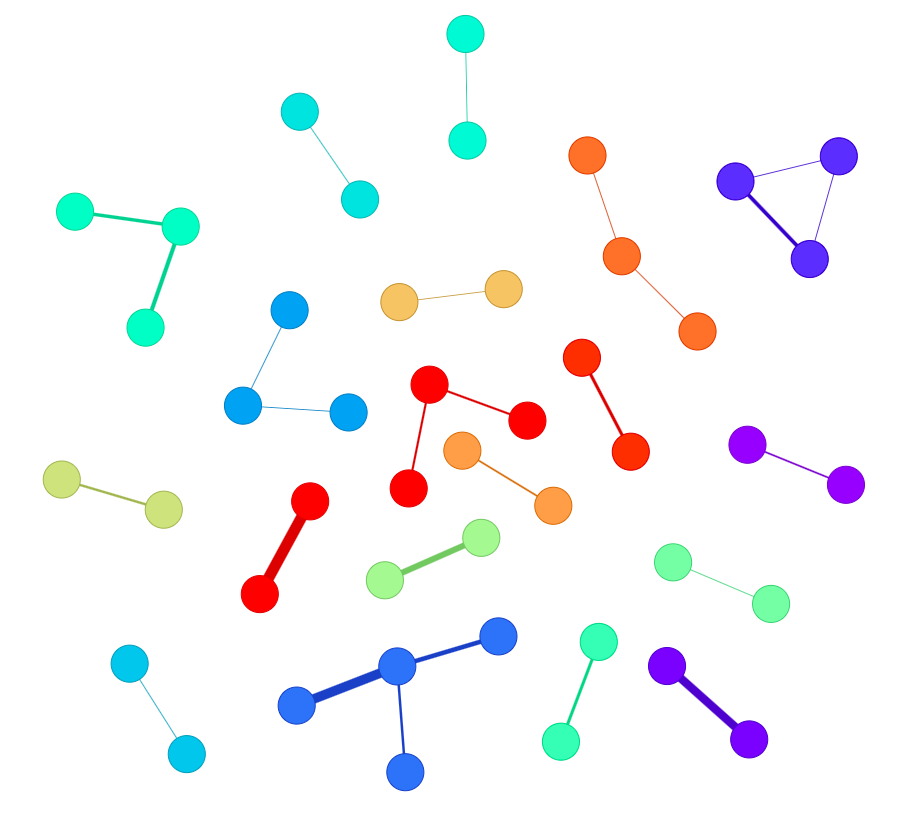
\includegraphics[width=\linewidth]{Minor Thesis/figures/graphs/main/g95202028.png}
		\caption{20\% cases min.}
	\end{subfigure}
	\hfill
	\begin{subfigure}[b]{0.30\linewidth}
		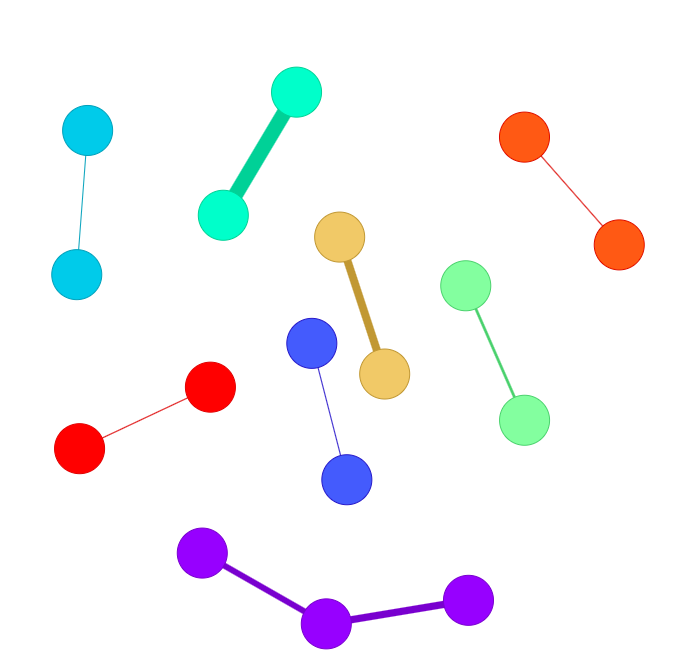
\includegraphics[width=\linewidth]{Minor Thesis/figures/graphs/main/g95302028.png}
		\caption{30\% cases min.}
	\end{subfigure}
	\hfill
    \caption{Rival variants graph. Each edge indicates the Strength Score among two variables. Colonies on Rivalry Score minimum = 0.95, 0.2 < Correlation < 0.8. (a) Discards variables whose original values are different less than 10\% of the feature's mode value, (b) does it on < 20\% and (c) on 30\%.}
    \label{fig:main-graphs}
\end{figure}

As we increase the Rivalry Score and the quasi-constant threshold, the results we get are fewer. After generating the new relations file, i.e. establishing rivalry relations among variables, and hence grouping them when counting, we proceed to re-rank the list. As seen in Table \ref{tbl:summary-exps}, the changes highly depend on the strictness of the thresholds. 

\begin{table}[!h]
\centering
\resizebox{\textwidth}{!}{%
\begin{tabular}{|c|c|c|c|c|}
\hline
\rowcolor[HTML]{EFEFEF} 
\textbf{Rivalry Score}  & \textbf{Quasi-constant leave-out index} & \textbf{Rank Changed} & \textbf{New in Top} & \textbf{New Top Total} \\ \hline
                        & 0.1                                     & 19                    & 4                   & 302                    \\ \cline{2-5} 
\multirow{-2}{*}{1}     & 0.2                                     & 2                     & 0                   & 298                    \\ \hline
                        & 0.1                                     & 62                    & 23                  & 321                    \\ \cline{2-5} 
\multirow{-2}{*}{0.975} & 0.2                                     & 15                    & 4                   & 302                    \\ \hline
                        & 0.1                                     & 146                   & 77                  & 375                    \\ \cline{2-5} 
                        & 0.2                                     & 46                    & 22                  & 320                    \\ \cline{2-5} 
\multirow{-3}{*}{0.95}  & 0.3                                     & 18                    & 9                   & 307                    \\ \hline
\end{tabular}%
}
\caption{Rank changes on different parameters of swapper results. Quasi-constant index indicates the percentage of values different from the feature's mode minimum required (0.1 = 10\%). Rank changed depicts how many nodes have changed their rank in the list, according to the new relations. Some features have entered the old top298 group which hold more than 8 votes, therefore the result set increases and some features are re-ranked gaining relevance.}
\label{tbl:summary-exps}
\end{table}
\\

Analysing the results, we observe the correlation among variables tend to be quite low (Figure \ref{fig:main-hist}). The Quasi-constant Leave-Out Index trims the node presence in the graph, however, it has no effect on correlation among variables. As a post-process step, we consider only the variables which hold a correlation close to 0.5, based on the fact that identical features containing quasi-constant values will have a correlation close to 1, and opposite features again containing quasi-constant values will have a correlation close to 0.
\\

\begin{figure}[!h]
    \centering
    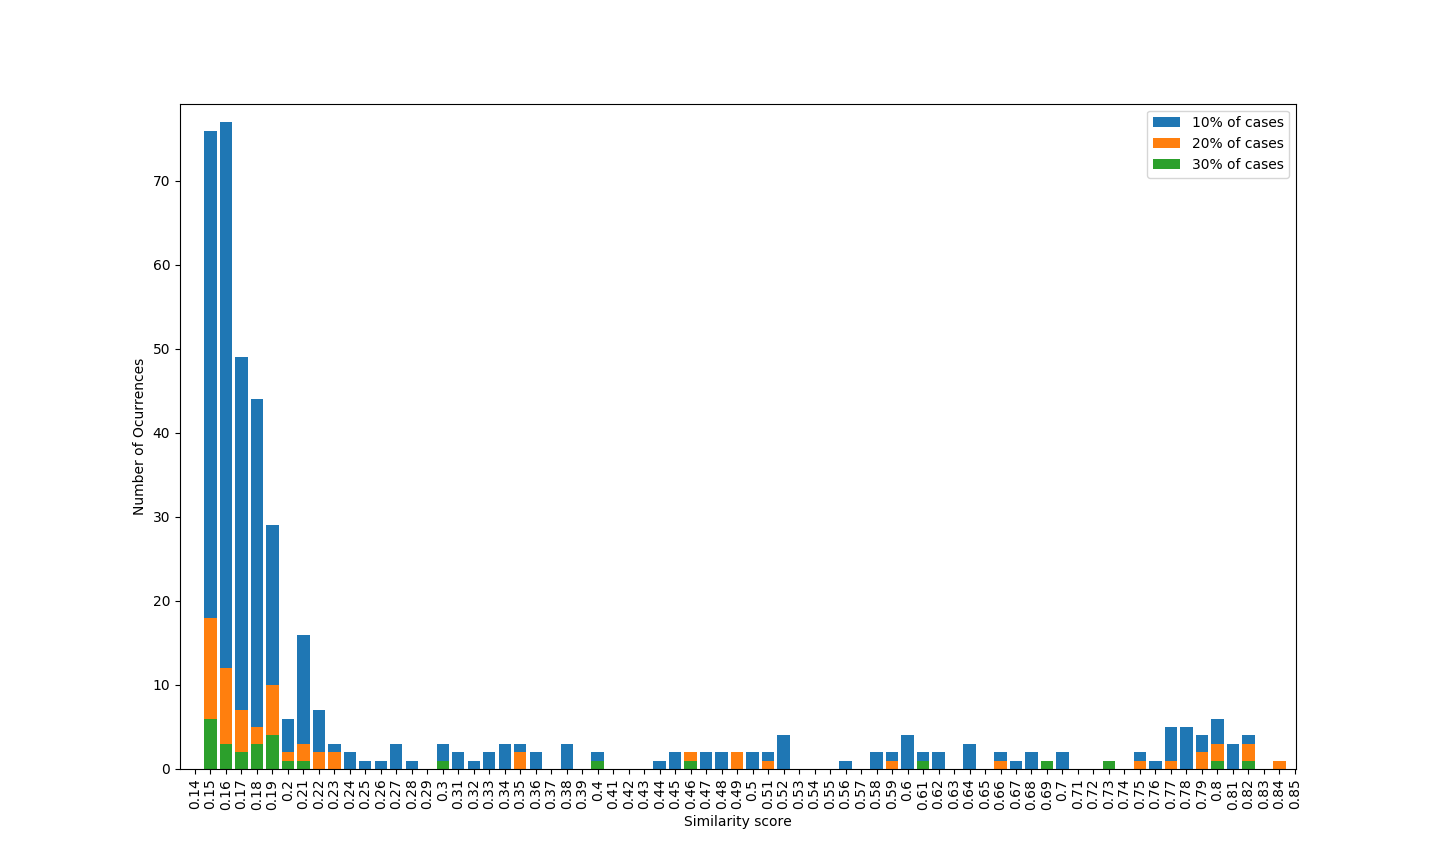
\includegraphics[width=0.75\linewidth]{Minor Thesis/figures/graphs/hist/Hist95.png}
    \caption{Spearman Correlation histogram of graphs from Figure \ref{fig:main-graphs}.}
    \label{fig:main-hist}
\end{figure}

Further analysis on Rivalry Scores of 0.975 and 1 can be found in Suppl. Material \ref{section:suppl:extra-hist}.